%%This is a very basic article template.
%%There is just one section and two subsections.
\documentclass[a4paper,12pt]{article}
\usepackage[T2A]{fontenc} 
% \usepackage[cp1251]{inputenc}
\usepackage[utf8x]{inputenc}
\usepackage[english,russian]{babel}
\usepackage{amssymb,amsfonts,amsmath,mathtext,cite,enumerate,float}
\usepackage{hyperref}
\usepackage{cite}

\usepackage{indentfirst} 

\usepackage{graphicx} 
\graphicspath{{./img/}}

\usepackage{pstricks-add}

\usepackage{xcolor}
\newcommand\TODO[1]{\textcolor{red}{\textbf{TODO}: #1}}


\title{Современная экономическая система России} % Заглавие документа
\author{Федор Вомпе, 507 группа}
\date{\today} % Дата создания


\begin{document}

\maketitle

\section{Введение}

Несмотря на рецессию в 2009 году, среднегодовой темп роста экономики России за
последние 12 лет составил более 5\% в год\cite{TheEconomist}. По данным
Организации экономического сотрудничества и развития 
\footnote{ \textbf{Организация экономиического сотруудничества
и развиития} (сокр. ОЭСР, англ. Organization for Economic Co-operation and
Development, OECD) — международная экономическая организация развитых стран,
признающих принципы представительной демократии и свободной рыночной экономики.
- \textit{источник
\href{http://ru.wikipedia.org/wiki/Организация экономиического сотрудничества
и развиития}{Википедия}} } темпы роста экономики России замедлятся 
до 4\% в этом и следующем году\cite{StandardPoor}. В то время как инфляция может
вырасти по сравнению 6,1\% в прошлом году\footnote{По данным
Росстата\cite{Rosstat} и журнала The Economist\cite{TheEconomist}}. Уровень
безработицы в настоящее время ниже среднего по данным ОЭСР.

В отличие от стойкого дефицита бюджета в 1990 году, за последние пару лет
в России наблюдается стойкий профицит бюджета. Все это благодаря
высокой и растущей цене за нефть, экономический росту, а также
благодаря налоговой реформе.

Целью этого эссе является исследование современной экономической
системы России, а также выявление основных экономических факторов, влияющих на
развитие экономики России. Основное внимание будет уделено структуре и динамике
ВВП России за последние несколько лет, т.к. в любой экономической системе
первичную роль играет производство в совокупности с распределением, обменом и потреблением.

\section{Структура экономики и тенденции развития экономики России}

Рост реального ВВП России в 2011 году составил 4\% и может составить эту же
цифру в нынешнем году в связи c усилением рисков замедления роста мировой
экономики, вызванных замедлением роста экономик США и Евросоюза, а также 
затянувшегося долгового кризиса в Европе и ожидаемого снижения цен на
нефть. \cite{WorldBank2011} \\
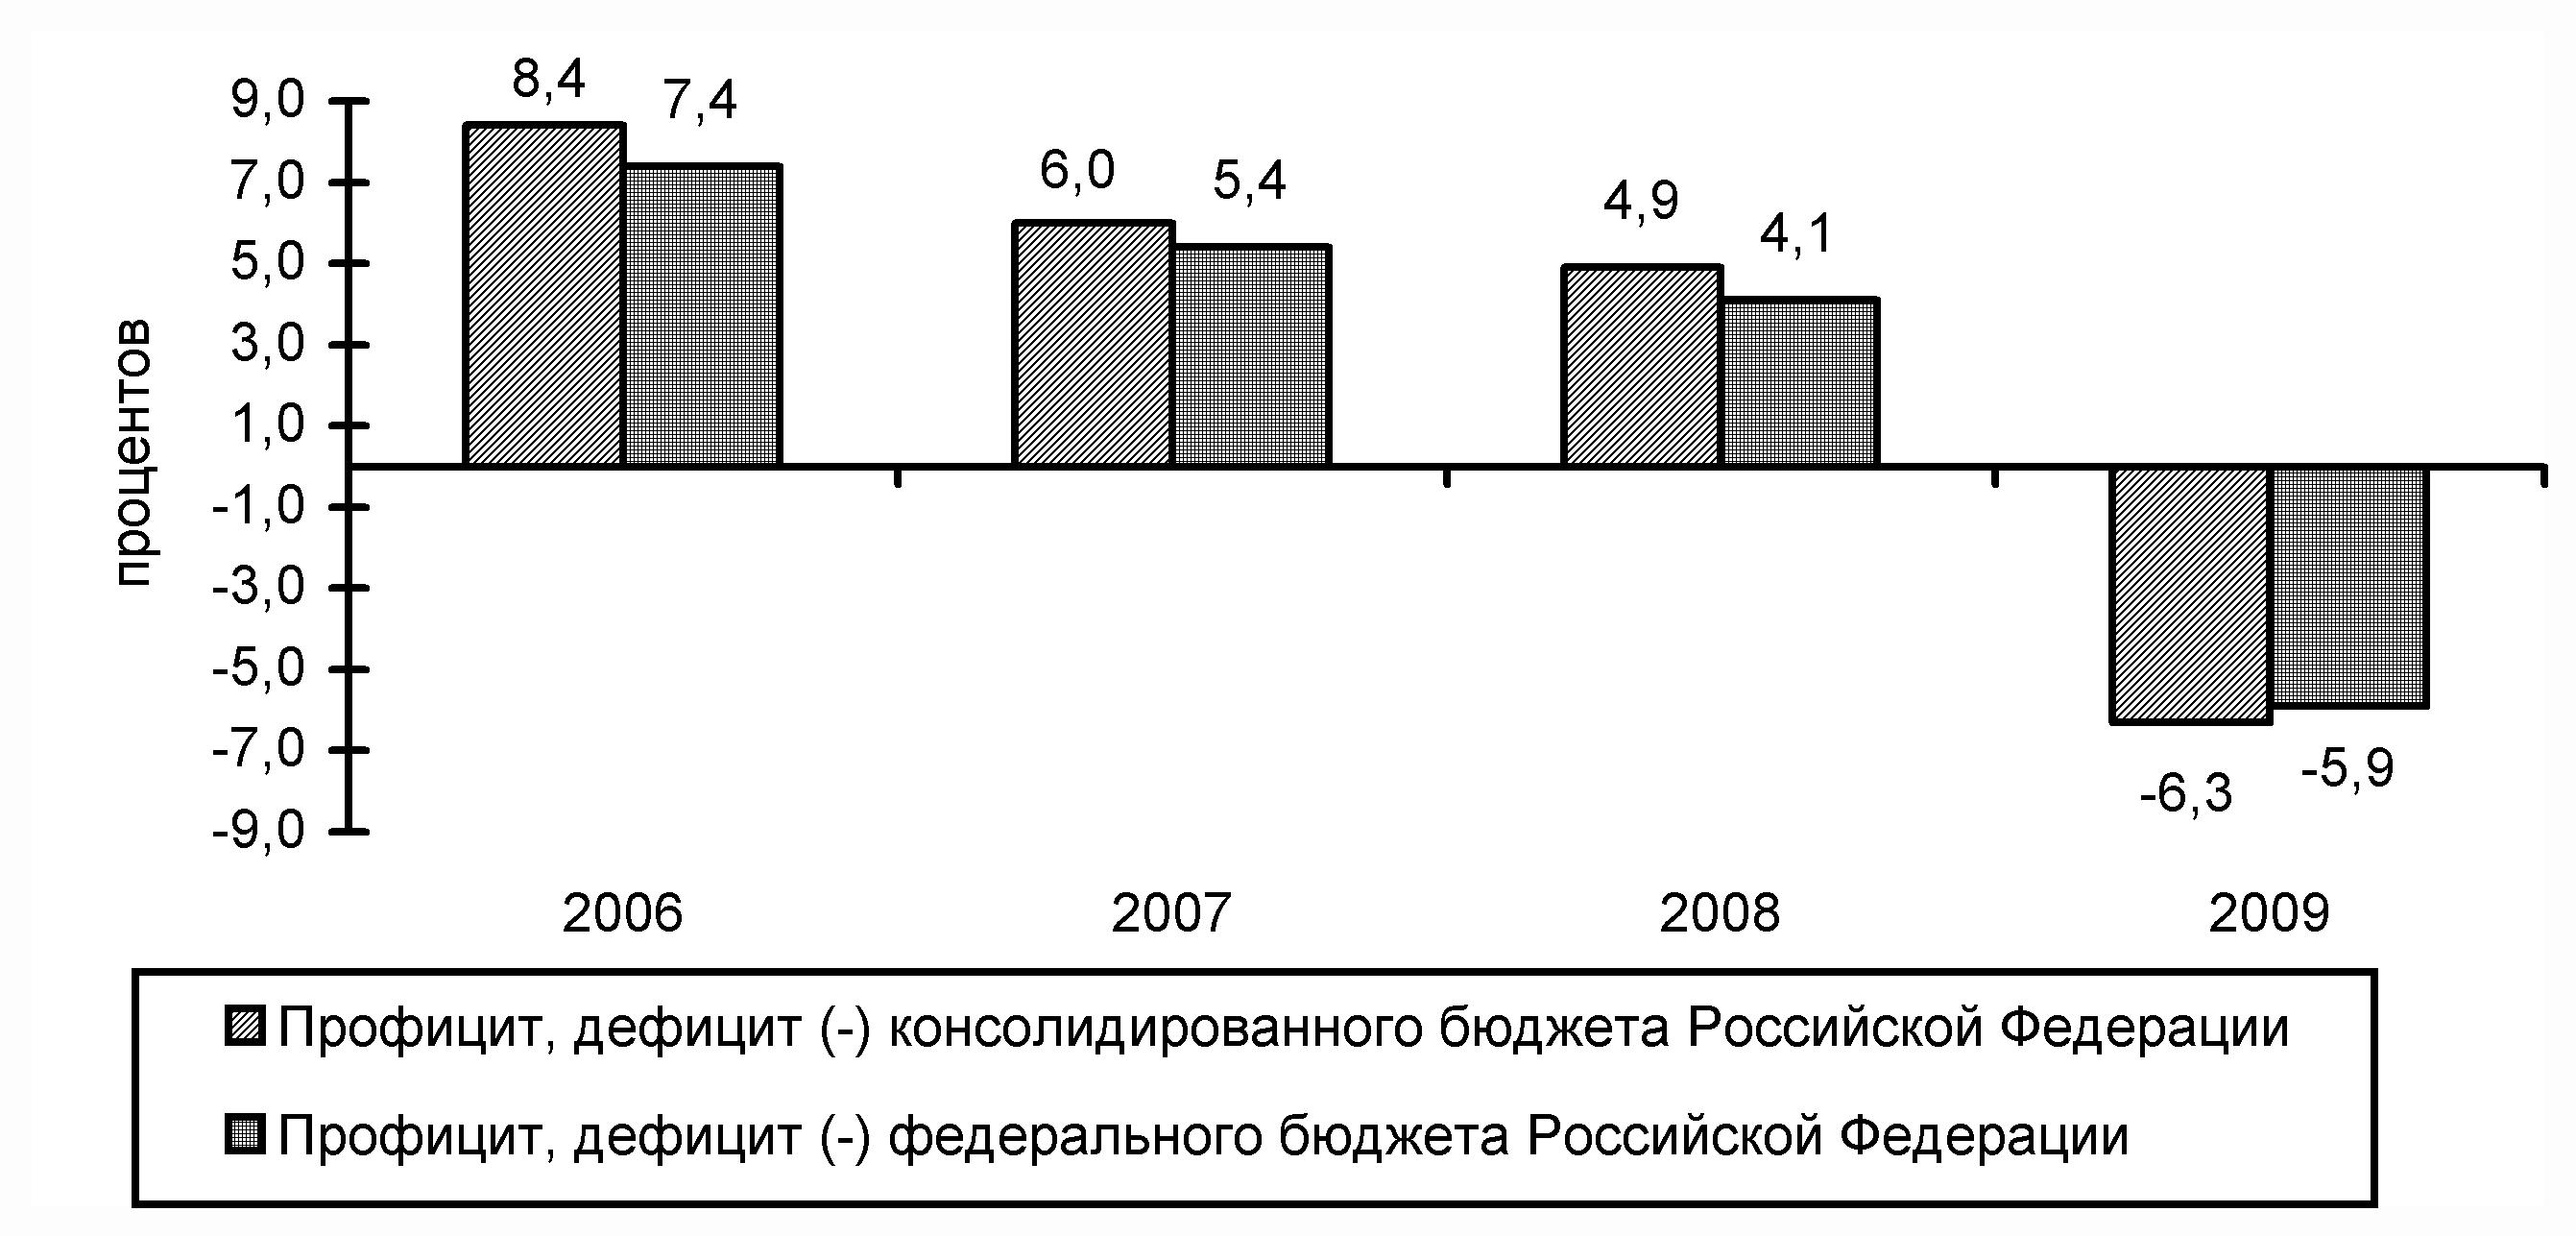
\includegraphics[width=1\textwidth]{Image3549.jpeg}
%По последним данным Росстата(на 2011 год) в структуре экономики России
%преобладает сектор услуг (торговля, транспорт, связь, финансовая деятельность,
%государственное управление, образование, здравоохранение, прочие слуги) 
%более 58,9 \% в ВВП. Этот показатель вырос примерно на 10\% с 2007 года.

Во время финансового кризиса 2009 года рост ВВП России составил отрицательную
величину -7.8\% по данным Всемирного банка в России и -6\% по данным Росстата.
Сельское хозяйство в 2010 рухнуло на 10\% по отношению к 2009 до минимумов с
2005. Единственный сектор, который не пострадал от экономического кризиса - это 
добывающая промышленность. Даже в кризис падения роста не было. Всего есть 6 
основных категорий, которые формируют ВВП России(в сумме 73.6\%
от ВВП) :
 добыча полезных ископаемых  (8.7\% от ВВП), 
 обрабатывающее производство (14.9\%), 
 розничная торговля (17.8\%), 
 транспорт (8.1\%), 
 операции с недвижимостью (9.2\%) и 
 налоги на продукты (14.9\%).

Среди всех отраслей промышленности России наиболее сильными, по отношению к 1991
году, выглядят: производство электрооборудования, электронного и оптического оборудования, 
химическое производство, обрабатывающие производства, добыча топливно-энергетических полезных 
ископаемых; целлюлозно-бумажное производство (лесные ресурсы России — крупнейшие в мире); 
издательская и полиграфическая деятельность; металлургическое производство и производство 
готовых металлических изделий; производство и распределение электроэнергии, газа
и воды (по данным на 2011 год).

Для понимания дальнейшего развития экономической системы России надо ответить
на вопрос о роли и влиянии новейших технологий. Сейчас идет пятый технологический уклад, 
он опирается на достижения в области микроэлектроники, информатики,
биотехнологии, генной инженерии, новых видов энергии, освоения космического пространства и т. п. 
Происходит переход от разрозненных фирм к единой сети крупных и мелких компаний, 
соединенных электронной сетью на основе Интернета, осуществляющих тесное взаимодействие 
в области технологий, контроля качества продукции, планирования инноваций. Стоит
отметить что по некоторым оценкам этот уклад начал формироваться в 1985 году и
будет продолжаться еще 50 лет.

Доля технологий пятого уклада в России составляет примерно 10\%, да и
то только в наиболее развитых отраслях: в военно-промышленном комплексе, в
авиакосмической промышленности. Более 50\% технологий относится к четвёртому
уровню, и около трети — к третьему. Отсюда понятна вся сложность стоящей
перед отечественной наукой и технологиями задачи: чтобы в течение ближайших 10 лет 
наша страна смогла войти в число государств с шестым технологическим укладом, 
ей надо, образно говоря, перемахнуть через этап — через пятый уклад.

Перемахнуть через пятый удастся только в том случае если наука будет обладать
статусом самостоятельной отрасли экономики. Ведущие страны мира к этому уже пришли.  
Большинство из них располагают мощным научным заделом, активной системой
инноваций, позволяющей создавать и постоянно поддерживать этот задел на высоком уровне, 
быстро превращая его в практические результаты.\cite{SixthTechn}

\section{Заключение}

Таким образом для того, чтобы динамично развивались и другие отрасли, в отличие
от добывающей промышленности, необходимо ввести дополнительные стимулы для
развития сфер образования, науки, новых технологий, а также отраслей
необходимых для полного перехода от прошедших технологических укладов к новейшему шестому укладу. 
Только изменение приоритетов в политике государства позволит укрепить и
модернизировать экономику Росии.

\bibliography{myrefs}{}   % expects file "myrefs.bib"
\bibliographystyle{plain} % (uses file "plain.bst")

\end{document}
